\documentclass[a4paper, 11pt]{article}

\usepackage[margin = 1in]{geometry} % for spacing around
\usepackage{graphicx} % for including images in your pdfs
\usepackage{xcolor} % for including colors in your pdf
\usepackage{soul} % for text decoration
\usepackage[utf8]{inputenc} % for encoded text
\usepackage[T1]{fontenc}
\usepackage{setspace} % for setting different line spacings between paragrafs.
\usepackage{enumerate} % for letting us get more detailed enumerate lists
\usepackage{multirow} % to let us combine more rows together
\usepackage{colortbl} % for decorating tables
\usepackage{amsmath} % used for representing more complicated math displays
\usepackage{supertabular}
\usepackage{longtable} % both of these packages are used to making really big tables
\usepackage{wrapfig} % allows us to wrap text around figures
\usepackage{fancyhdr} % for making fancy headers
%\usepackage{bibtex} % for making better bibliographies
\usepackage[pdftex]{hyperref} % for letting us make links
\usepackage{lscape} % Allows us to flip from portrait to landspace
\usepackage{tikz} % for high detailed drawing
\usepackage{multicol} % To put things side by side
\usepackage{rotating} % For rotating objects
% \usepackage{draftwatermark} % For adding watermarks
\usepackage{MnSymbol} % for using multiple symbols
\usepackage{mathtools} % Used for more math symbols
\usepackage{xfrac} % For more complciated fractions and to add derivitives
\usepackage{hyperref} % for hyper links
\usepackage{enumitem} % for better enum lists
\usepackage{tcolorbox} % for adding colored text boxes
\usepackage{bm} % Adding bold text to math inputs
\usepackage{unicode-math}

% Setting up the default image path
\graphicspath{{./Images/}}

% Implementing authro details
\title{CS103 Project Report \\ CodeLab Notes \\ \small{code-editor}}
\author{Emre Arapcic-Uvak & Vedad Siljic}
\date{}

% Setting up the fancy page style
\fancypagestyle{customStyle}{
	\lhead{} \chead{} \rhead{}
	\lfoot{} \cfoot{\thepage} \rfoot{}
	\renewcommand{\headrulewidth}{0pt}
	\renewcommand{\footrulewidth}{1pt}
}
\pagestyle{customStyle}

% Setting up hyperref options
\hypersetup {
	colorlinks = false,
	citecolor = black,
	filecolor = blue,
	linkcolor = blue,
	urlcolor = blue,
	pdftex
}

% Custom commands
\newcommand{\important}[1]{\textcolor{red}{\textbf{\textsc{#1}}}}
\newcommand{\miniHeader}[1]{\begin{large}\textbf{\textsc{#1}}\end{large}}
\newcommand{\volumeUnit}[0]{\frac{g}{cm^{3}}}

\def\checkmark{\tikz\fill[scale=0.4](0,.35) -- (.25,0) -- (1,.7) -- (.25,.15) -- cycle;} 

\begin{document}
	\begin{figure}
		\centering
		
\includegraphics[scale = 0.5]{IUS_Logo}
		\\ \vspace{5mm}
		\noindent \large{\textsc{International University of Sarajevo}}
	\end{figure}
	\maketitle
	\vspace{5mm}

	\begin{abstract}
		\noindent This is a \emph{brief} project report for CS103. This report will go over basic information of the program talking about its functionalities and abilities as a code editor, furthermore it will go over who went over what, what were the challenges that were face during the production of this program, and what were we able to learn from doing this project.
	\end{abstract}
	\pagebreak
	
	\tableofcontents
	\pagebreak
	
	\section{Assignments}
		\noindent The following table will show all the assignments taken by the corresponding students:
		\vspace{5mm}
		{
			\centering
			
			\begin{tabular}{|c|c|c|}
				\hline 
						& \textsc{Emre Arapcic-Uvak} & \textsc{Vedad Siljic} \\ \hline
				 Design &  x & \checkmark \\ \hline
				 Tree File Display & \checkmark & x \\ \hline
				 File Saving & \checkmark & x \\ \hline
				 File / Dir Creating & \checkmark & x \\ \hline
				 File / Dir Deleting & \checkmark & x \\ \hline
				 File Opening & \checkmark & \checkmark \\ \hline
				 Multi File Tab & \checkmark & \checkmark \\ \hline
				 Syntax Highlighting & x & \checkmark \\ \hline
				 Custom Text Widget & x & \checkmark \\ \hline
				 About Sections & \checkmark & \checkmark \\ \hline
				 Font Customization & x & \checkmark \\ \hline
				 Directory Model Management & \checkmark & x \\ \hline
	 		\end{tabular}
		
			\par
		}
	
		\section{Information about the program}
			\subsection{Program overview}
				\noindent The program \emph{\textsc{CodeLab Notes}} is a plain code editor that supports multiple file editing, and syntax highlighting for \textbf{c} and \textbf{cpp} files. \\
			
				\noindent Upon the start up of the program the user is greeted with an giant logo of the program as well as a tree view of the users root directory and a tool bar right above the tree view; right above the tool bar there are also drop down menus for even more options that are given to the user to choose from as all can be seen in Figure \ref{Fig:Program start screen}
				
				\begin{figure}[h]
					\centering
					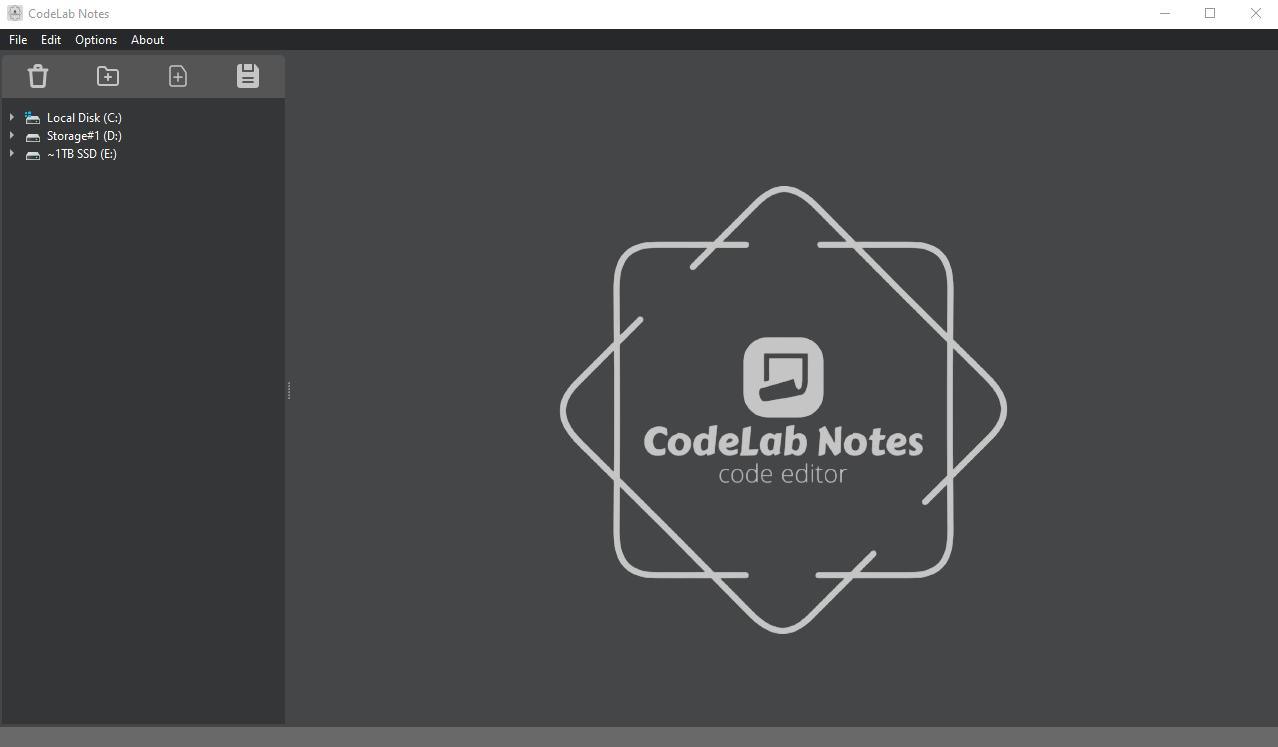
\includegraphics[scale = .4]{programStartScreen}
					\caption{Starting screen of CodeLab - Notes}
					\label{Fig:Program start screen}
				\end{figure}
			
			\subsection{Tree view and working directory}
				\noindent Like many other code editors CodeLab Notes has the ability to select a directory which the user will be working with. For the user to select a working directory all that they will have to do is go to the \emph{File} menu and select \emph{Open Folder} as can be seen in Figure \ref{Fig:Open Folder option in CodeLab Notes}
				
				\begin{figure}[h]
					\centering
					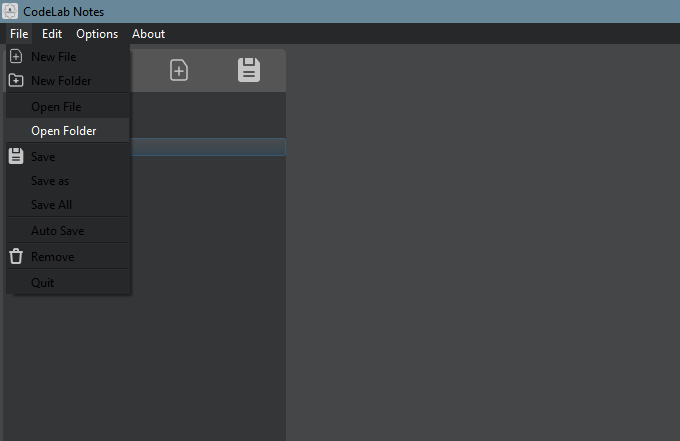
\includegraphics[scale=.7]{openFolderOption}
					\caption{Open Folder option in CodeLab Notes}
					\label{Fig:Open Folder option in CodeLab Notes}
				\end{figure}
			
				\noindent Upon selecting this option the user will be prompted a directory dialog which asks the user to select what folder they would like to open; afterwards the tree view will update such that it only displays the selected directory as can be seen in Figure \ref{Fig:Directory prompt dialog} and Figure \ref{Fig:Tree view update}.
				
				\begin{figure}[h]
					\centering
					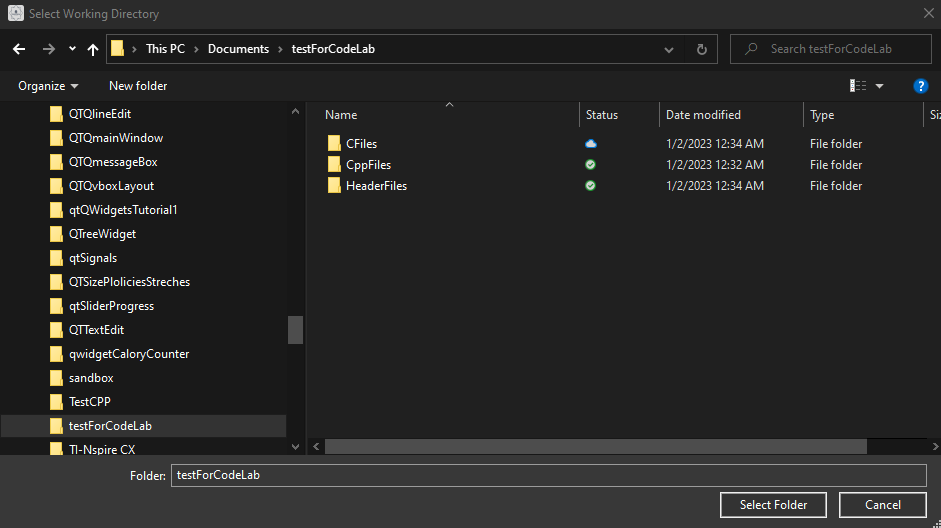
\includegraphics[width = .9\linewidth]{directoryDialogPromt}
					\caption{Directory prompt dialog}
					\label{Fig:Directory prompt dialog}
				\end{figure}
				\pagebreak
				
				\begin{figure}[h]
					\centering
					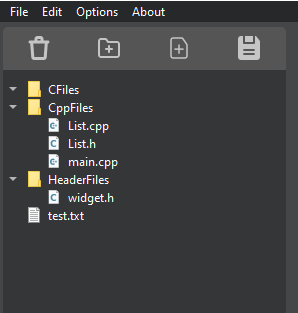
\includegraphics[width = .3\linewidth]{updatedTreeView}
					\caption{Tree view update}
					\label{Fig:Tree view update}
				\end{figure}
			
			\subsection{Opening and Modifying files}
				\noindent To open files all that has to be done is to is to double click on a file in the tree view, or select the open file option from the file menu which will open the text editor where the logo is, and give you tabs on the top of the text editor as can be seen in Figure \ref{Fig:Opened Files}
				
				\begin{figure}[h]
					\centering
					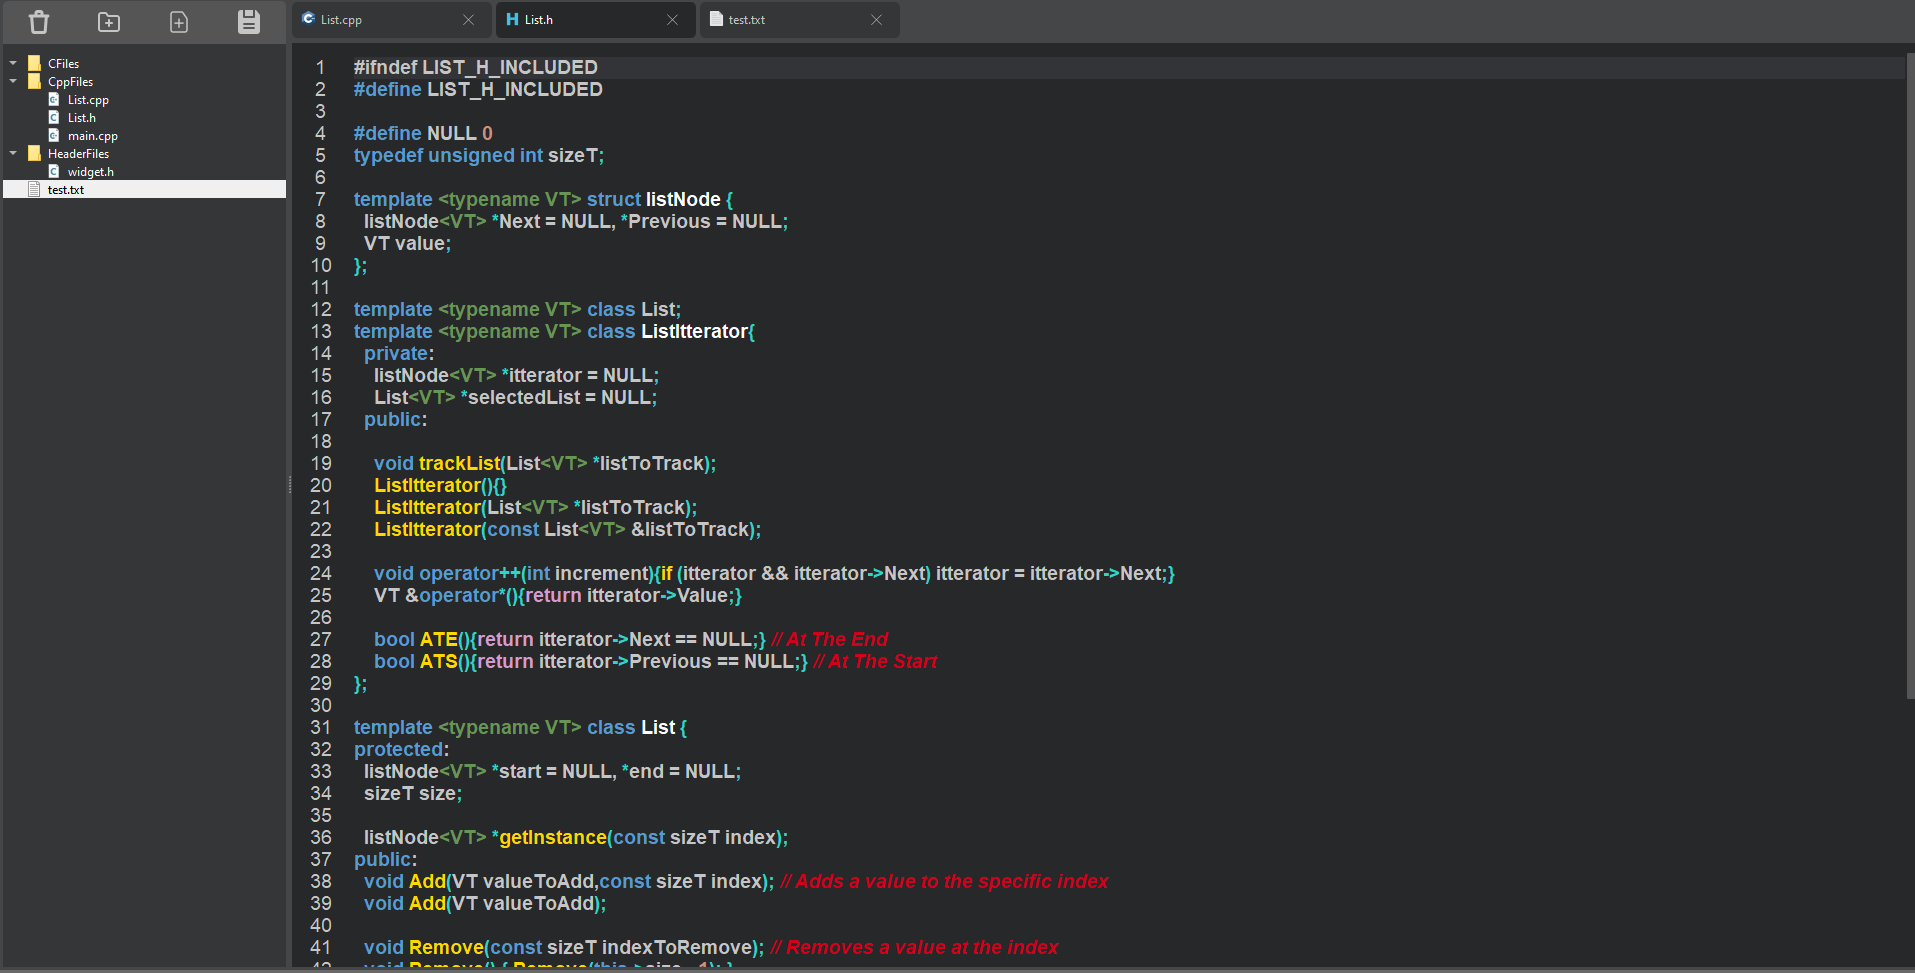
\includegraphics[width = \linewidth]{openedFiles}
					\caption{Opened files in CodeLab Notes}
					\label{Fig:Opened Files}
				\end{figure}
			
				\noindent As we can also see CodeLab Notes also has its own syntax highlighting. One key feature of any code editor or any text editor in this matter is the ability to save your work. CodeLab Notes has four saving features and those are:
				\begin{enumerate}
					\item Save
					\item Save As
					\item Save All
					\item Auto Save
				\end{enumerate}
			
				\noindent Save and Save all are pretty self explanatory, Save saves the file currently focused and Save all save all files that have been opened. Auto Save is a feature that automatically saves your file when u go to another tab or open another file, and Save As saves your files but prompts you a dialog similar to the dialog that can be seen in Figure \ref{Fig:Directory prompt dialog} but this time it asks you where do you want to save the file and under what name and extension. \\ \vspace{1mm}
				
				\noindent Deleting files/directories is also a possibility, all that has to be done is select what file / directory you want to delete in the tree view and press on the delete button in the tool bar or in the file menu; because the tool bar is just a faster way to get all the settings from the file menu.
				
			\subsection{Text editing features}
				\noindent If we take a look in the \emph{Edit Menu} we can see a lot of useful feature the users are given, and those features are:
				\begin{itemize}
					\item Undo
					\item Redo
					\item Cut
					\item Copy
					\item Paste
				\end{itemize}
			
				\noindent A lot of these are self understandable but we will cover them briefly. Undo undoes any recent changes done to a file, redo does the exact same, cut cuts text and saves it into the clip board, copy copies selected and saves it into the clip board, and paste puts the text from the clip board into the text editor.
\end{document}